\begin{figure*}
\centering
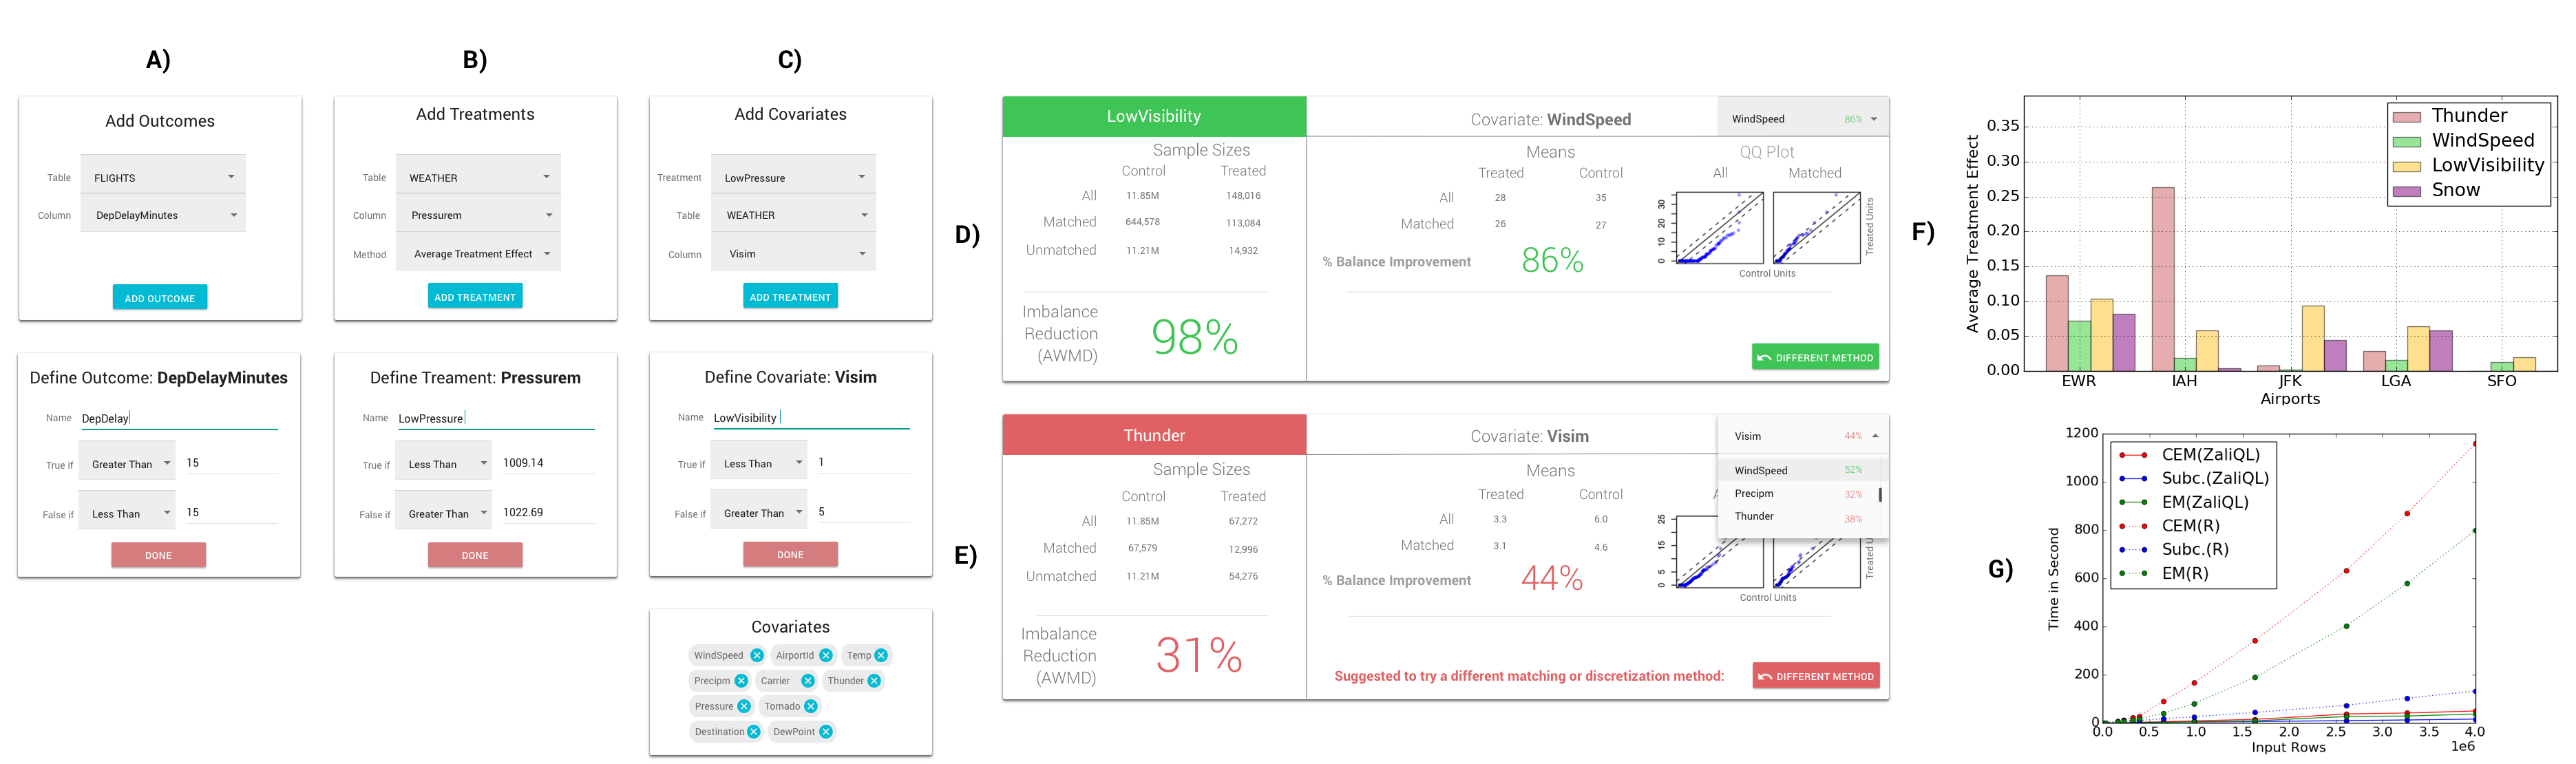
\includegraphics[scale=0.13]{Figures/Demo-Tutorial-2.png}
\caption{Demonstration screenshot described in section \ref{sec:dd}}
\label{sfig:demo-tutorial}
\end{figure*}


\section{Demonstration Details}
\label{sec:dd}
Modern causal analysis is an iterative process, as we illustrate in Fig \ref{fig:flowchart}.
One generates a hypothesis, pre-processes  relevant data with matching (explained below),
  then conducts the causal analysis; most often this needs to be repeated with a new matching
  method, a new hypothesis or  new datasets.
We demonstrate \GSQL\ by showing several real causal analysis performed on two,
  large datasets that we downloaded from the Web and integrated in Postgres.

\ignore{
 In this demonstration, we will use \GSQL\ to quantify the causal effect of
 different weather conditions on flight departure delay. }

    {\bf Data:} The analysis will be conducted on a spatio-temporal join of the following datasets:
(a) {\it Flight dataset (105M entries)}: collected by the US
Department of Transportation.\footnote{\url{http://www.transtats.bts.gov/}} It contains
records of more than 90\% of US domestic flights of major airlines
from 1988 to the present. It includes attributes such as FlightDate, OriginAirportID,
CarrierID, CRSDepTime (scheduled departure time), and DepDelayMinutes (departure delay).
(b) {\it Weather dataset (40M entries):} historical weather data for relevant flight gathered using the Weather Underground API.\footnote{\url{https://www.wunderground.com}} It includes Code (Airport ID),
Date, Time,  Visim (visibility in km),
  Tempm (Temperature in C$^{\circ}$)
  Wspdm (wind speed kph), Pressurem (Pressure in mBar), Precipm  (Precipitation in mm), Snow (binary), Thunder (binary).






\ignore{
\begin{figure*}
\begin{subfigure}{0.50\linewidth}
\centering
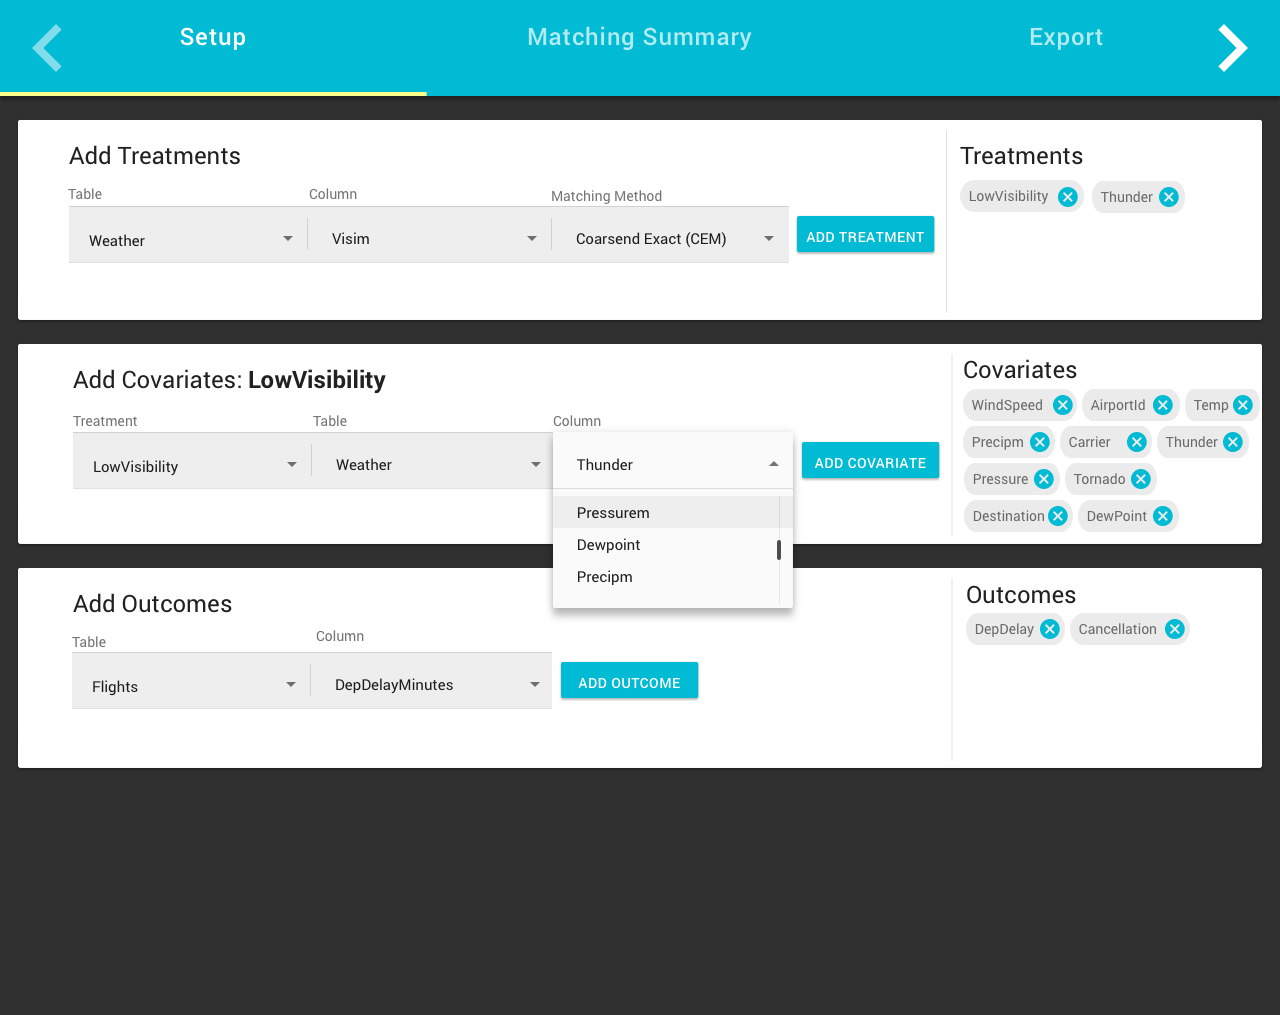
\includegraphics[scale=0.13]{Figures/Setup.png}
\label{sfig:testc}
\end{subfigure}\hfill
\begin{subfigure}{0.47\linewidth}
\centering
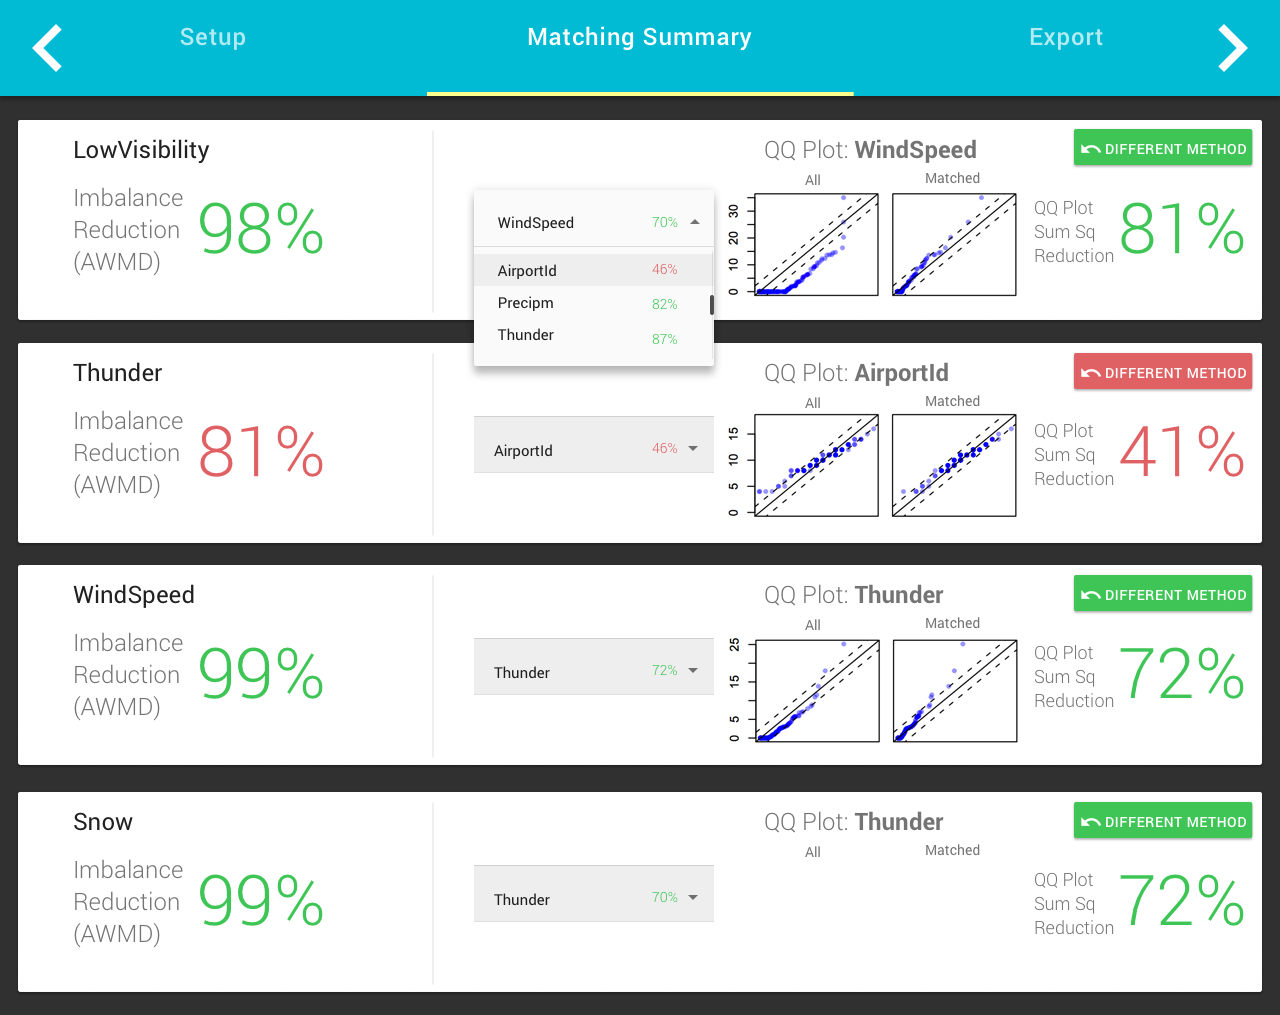
\includegraphics[scale=0.13]{Figures/Matching-Summary.png}
\label{sfig:testd}
\end{subfigure}\hfill
\caption{Demonstration Screenshot described in Section \ref{sec:dd}}
\label{fig:eteresult}
\end{figure*}
}









 \ignore{
 The analysis will be conducted on
 {\em flight data (105M eateries)}-collected by the US Department of Transportation (U.S. DOT)- and  {\em weather dataset} (10M eateries)-gathered using the weather underground
API. }

 \ignore{
 The {\em flight dataset} we use was collected by the US Department of Transportation (U.S. DOT) \cite{flightdata}. It contains
records of more than 90\% of US domestic flights of major airlines
from 1988 to the present. The {\em weather dataset} was gathered using the weather underground
API \cite{Weatherdata}.  \ignore{Its attributes are also presented in Table
\ref{tab:attlist}. In addition, we pre-computed two other attributes
AiportTraffic and CarrierTraffic. The former is the total number of
flights occur in the origin airport of a flight one hour prior to the
flight departure time, the latter is the same quantity restricted to
the flights from the same carrier.  We managed to acquire and clean
35M weather observations between 2000 and 2015.} These datasets are
integrated by a spatio-temporal join.}



\ignore{

        \caption{Weather dataset}
    \end{subtable}
 \vspace{-0.1cm}   \caption{\bf{List of attributes from the flight(a) and weather(b)  datasets that are relevant to our analysis.}}
\label{tab:attlist}
\end{table}
}









\ignore{
\begin{example} \em \delay (cont.) \ \em   Suppose we want to explore the effect of the low-pressure (treatment) on flight departure delays (outcome).  The direct comparison of
delay between flights that happen during low-pressure (treated groups) and opposite (control group) is misleading.  It is known that high pressure is generally associated with clear weather,    while low-pressure is associated with unsettled weather, e.g.,
    cloudy, rainy, or snowy weather\ignore{\cite{weba2,barometricpressureheadache:article}}. Thus, as shown in Figure \ref{fig:cv}, factors such as thunder, snow, visibility confound pressure and delay. Therefore, conducting any sort of predictive analysis identifies
    low-pressure as a predictor for flight delays.
  However, low-pressure does not have any causal impact on departure delay
    (low-pressure only requires longer takeoff distance) \cite{FAA08}. In this demonstration, by conducting a careful causal analysis using \GSQL, we show that low-pressure is only a correlated attribute with flight delays and has no significant causal impact on flight delay.

    \ignore{By performing a careful casual analysis
    \GSQL\ found that other attributes such as thunder, low-visibility, high-wind-speed and
    snow have the largest causal effect on flight delays (see Sec. \ref{sec:endtoend});
  this is confirmed by the results reported by the FAA.}
\end{example}
}

 {\bf Causal Questions:} Our demonstration starts by creating a set of {\em causal questions} regarding the effect of different weather attributes on flight delays.
Q1: Does low air pressure causes flight departure delays?
Q2: Which weather features have the main causal effect on departure delays?
Q3: Do the findings to the previous question differ between major aiports? We answer these questions using \GSQL\ by

\begin{enumerate}
  \item specifying DepDelay as our outcome of interest (potential effect)
as shown in Figure \ref{sfig:demo-tutorial}(a)
  \item specifying a set of binary treatments (potential causes) that might affect DepDelay,
 as shown in Figure \ref{sfig:demo-tutorial}(b),
In particular the following binary treatments will be created:
 LowVisibility (1 if Visim$<1$; 0 if Visim$>5$); \
  HeavySnow (1 iff Precipm$>0.3$ and Snow$=1$); \
  WindSpeed (1 if Wspdm$>40$; 0 if Wspdm$<20$); \
  Thunder; \ LowPressure (1 if Pressurem$<1009.14$; 0 if Pressurem$>1022.69$)     \ignore{
      As shown in Figure \ref{sfig:demo-tutorial}(b) Clicking on the {\it ADD TREATMENT}, {\it ADD COVARIATE}, and {\it ADD OUTCOME} buttons will trigger a dialog allowing
  further customization on the discretization and matching methods.
These dialogs will also allow the user to incorporate other columns (e.g. snow is defined as $iff Precipm> 0.3 and
Tempm< 0$) and input SQL for custom discretization methods.}
    \item specifying a subset of data that is relevant to the analysis.  We select five US airports  with high rate of weather-related delay, namely, San Francisco (SFO) , John F. Kennedy (JFK), Newark Liberty (EWR), George Bush (IAH), and LaGuardia Airport (LGA).
\end{enumerate}

\ignore{
(1) specifying DepDelay as our outcome of interest (potential effect)
as shown in Figure \ref{sfig:demo-tutorial}(a),
(2) specifying a set of binary treatments (potential causes) that might affect DepDelay,
 as shown in Figure \ref{sfig:demo-tutorial}(b),
In particular the following binary treatments will be created:
 LowVisibility (1 if Visim$<1$; 0 if Visim$>5$); \
  HeavySnow (1 iff Precipm$>0.3$ and Snow$=1$); \
  WindSpeed (1 if Wspdm$>40$; 0 if Wspdm$<20$); \
  Thunder; \ LowPressure (1 if Pressurem$<1009.14$; 0 if Pressurem$>1022.69$)     \ignore{
      As shown in Figure \ref{sfig:demo-tutorial}(b) Clicking on the {\it ADD TREATMENT}, {\it ADD COVARIATE}, and {\it ADD OUTCOME} buttons will trigger a dialog allowing
  further customization on the discretization and matching methods.
These dialogs will also allow the user to incorporate other columns (e.g. snow is defined as $iff Precipm> 0.3 and
Tempm< 0$) and input SQL for custom discretization methods.} and (3) specifying a subset of data that is relevant to the analysis.  We select five US airports  with high rate of weather-related delay, namely, San Francisco (SFO) , John F. Kennedy (JFK), Newark Liberty (EWR), George Bush (IAH), and LaGuardia Airport (LGA).
}


 { \bf Computing ATE}: In causal inference, the objective is to quantify
 the causal effect of a binary attribute called treatment, on an attribute called outcome.
 A common measure to to compute causal effect is {\em average treatment effect (ATE)}, which is defined as the difference in expected values of the treated and untreated units.\footnote{In causality literature subjects of a study,
  e.g., patients in a clinical trial, are called units. In our case each flight
   is considered a unit.}\ignore{\dans{this part is good.
    But I would make it a bit more tutorial-style.  Start by
    saying that in causal analysis we want to study
    the causal effect of a binary attribute called treatment, on an attribute
    alled outcome.  The ATE is defined as the difference in expected
    values of the treated and untreated units.
    (Add a footnote saying that records are called units in causal analysis).
     Then continue with what you have here, by referring to Q1 above:} } For example for Q1, \GSQL\ computes ATE as $$E[\text{Depdelay}|\text{LowPressure}=1] - E[\text{Depdelay}|\text{LowPressure}=0]$$
  where, E[\text{Depdelay}|\text{LowPressure}=$x$], $x=(0,1)$ is
  computed by taking the emetical average of  Depdelay where LowPressure is  $x$.
  It is a  common measure to compare an
  outcome (DepDelay) in the {\em treated group},  those subjects
  (flights) that receive a treatment (LowPressure=1), with the {\em control group}, the opposites.
\ignore{\dans{For the next sentence, can you refer to Fig. 3.
  There the user has selected the treatment visibility (Visim)
   and the outcome is DepDelayMinutes.  (Acually, can you update
    the figure so that the treatment is LowPressure).  If we compute
    the ATE for LowPressure on DepDelay, the result is  (give concrete number).}}  We show that for LowPressure, ATE is 3.7min, which is a relatively large that suggests pressure it affects DepDelay. However, it is known that
  LowPressure does not have any causal impact on departure delay (it only requires longer takeoff distance) \cite{FAA08}. This observation raises the question that  where does this difference coming from?


%%%%%%%%%%%%%%%%%%%%%%%%%%%%%%%%%%%%%%%%%%%%%%%%%%%%%%%%%%%%%%%%%%%%%%%%%%%%%%%%%%% check ba;ance


\ignore{
 \paragraph{\bf Confounding variables:} \dans{Use this as an excuse to continue the mini-tutorial.  The first 1-2 setnences should be general, saying that  causal analysis conditions on confounding variables. Then you immediately make it concrete and say that, if the confounding variable is LowVisibility, then the ATE for LowPressure on DepDelay decreases significantly.} We address this question, by demonstrating that the comparison of DepDelay between the treated and control groups is misleading due to the existence of the so-called {\em  confounding influence} of other variables such as visibility, snow and thunder.  In fact we show that, LowPressure is highly associated with unsettled weather conditions such as LowVisbility. For instance the average of LowVisbility in the treated group is much less than
  the opposite group. Thus, it is unclear that the observed DepDelay difference between the groups is causes by LowPressure or LowVisbility. This scenario, as shown graphically in Figure \ref{fig:cv}, demonstrates that in the presence of {\em confounding variable} (a.k.a, {\em covariates}) the treated and control groups are very different and comparing them without accounting for the confounding variables could be misleading.
}

\ignore{ \dans{Use this as an excuse to continue the mini-tutorial.  The first 1-2 setnences should be general, saying that  causal analysis conditions on confounding variables. Then you immediately make it concrete and say that, if the confounding variable
  is LowVisibility, then the ATE for LowPressure on DepDelay decreases significantly.}}
 {\bf Confounding variables:} The main issue with causal inference from observational data
 is the exitance of {\em confounding variables} that  make it difficult to establish a clear causal link between treatment and outcome.   We show that the observed positive effect of LowPressure
 was the result of the confounding influence of other variables such as visibility, snow and Thunder
    Specifically, we show that, LowPressure is highly associated with unsettled weather conditions such as LowVisbility. For instance the average of LowVisbility in the treated group is much less than
  the opposite group. Thus, it is unclear that the observed DepDelay difference between the groups is causes by LowPressure or LowVisbility.


\ignore{
  This scenario, as shown graphically in Figure \ref{fig:cv}, demonstrates that in the presence of {\em confounding variable} (a.k.a, {\em covariates}) the treated and control groups are very different and comparing them without accounting for the confounding variables could be misleading.
}
\begin{figure}
\hspace*{.3cm}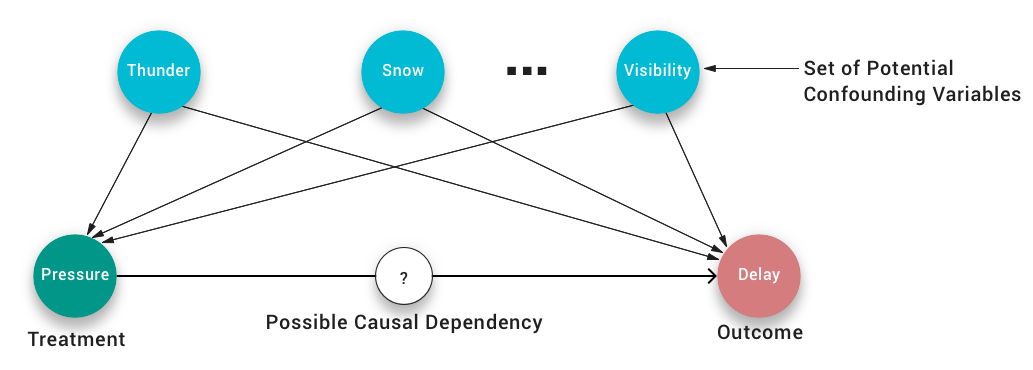
\includegraphics[scale=0.2]{figures/Scenario-Graph.png}
\caption{Confounding influence}

\label{fig:cv}
\vspace{-0.3cm}
\end{figure}
 {\bf Adjusting for confounding variables:} {
Causal inference provides a framework for adjusting for the effects of
confounding variables.
 With only one categorical confounding variable, adjustment can be
 done simply by partitioning data into
 groups with similar values of the confounding variable, then
 computing the ATE as  weighted average of average treatment effects in each groups. However, real-world causal analysis requires a dozen or more continues confounding variables, and in this case there is not enough data in each group to enable a meaningful estimation of the ATE. For example, as exemplified in Figure \ref{fig:cv}, LowPressure has more than ten confounding variables.  Most of the complexity in causal analysis tools, as well as in \GSQL, consists of implementing sophisticated methods for enlarging the groups while still performing a meaningful inference of the ATE.
 \ignore{\dans{I would start this paragraph by saying that, using a single confounding variable is easy, since we essentially partition the data into two groups.  But real-world causal analysis requires a dozen or more confounding variables, and in this case there is not enough data in each group to enable a meaningful estimation of the ATE. For example, refer to Fig 2 to show a more complex set of confounding variables.  Most of the complexity in causal analysis tools, as well as in \GSQL, consists of implementing sophisticated methods for enlarging the groups while still performing a meaningful inference of the ATE.  Then continue with:}}
}

\GSQL\ controls for confounding influences (a task usually referred to
as {\em covariate adjustment}) using {\em subclassification} and {\it propensity score matching} \cite{Rubin1983b,IacKinPor09,rosenbaum1984reducing}.
These are popular methods for covariate adjustment developed in social
science and statistics. We refer to these as matching methods.
The key goal of matching is to prune data so that
the remaining data ({\em matched data}) have better \emph{balance}
between the treated and control groups. That is, the empirical
distributions of the confounding variables in the treated and control
groups are similar after matching.
Once the two groups are balanced, any observed difference of the
outcome between the two groups can be attributed to the treatment. In
our demo,
\begin{enumerate}
  \item for each treatment, we select a set of covariates deemed to confound the treatment and DepDelay (Figure \ref{sfig:demo-tutorial}(d)).
  \item we select a matching method and adjust its tuning parameters (Figure \ref{sfig:demo-tutorial}(e)).
\end{enumerate}


{\bf Checking Balance:}  In this step, we check whether the
matching process  successfully improved the covariates' balance. In particular,
(1)  we compare the distribution for each covariate between the treated and control group on matched data (this will be done for all treatments). For this task, \GSQL\  provides numerical summaries such as the mean difference and visual summaries such as quantile quantile plots \ref{sfig:demo-tutorial}(d,e).
(2)  we can perform different matching methods using different
        parameters, showing that different methods trade off balance and size of matched data% to demonstrate the advantages and disadvantage of different methods.

      The main objective of this step is to demonstrate the typical workflow of
       causal inference from observational data.
        As shown in Figure \ref{fig:flowchart}, it
        consists of the iterative process of matching and balance checking. This highlights the demand for tools such as \GSQL\, which perform matching at scale.

     {\bf Answer to the causal questions:} %\dans{We should give here concrete answers to the queries Q1,Q2,Q3.  Then add a sentence saying that we will perform other causal analysis during the demo}
In this step,  we answer the causal questions created at the very first step of the demonstration using
\GSQL. For Q1, we show that LowPressure has no significant causal effect on DepDelay.
For Q2, we identify that other treatments have significant causal effect on DepDelay
 (Figure \ref{sfig:demo-tutorial}(F)).
   \ignore{
       \item for each treatment we compute ATE on the associated balanced matched data
      \item we evaluate the statistical significance of the obtained
        result by performing statistical tests, such as the chi-square test.
          \item For Q3 we report the major causes of flight delay at the airports under study.}
For Q3, we report the major causes of flight delay at the airports under study are
     actually different. We show that the obtained results are in accordance with
FAA reports. % \footnote{\url{https://www.faa.gov/}}
For example, the runway configuration at SFO makes the airport
unusually susceptible to delays in low-visibility conditions~\cite{faa-sfo}.
% which reported the following major weather-related
% causes:
% snows, thunders and wind at EWR; thunder and fog at IAH;
% snows and visibility at JFK; snows at LGA; visibility at SFO;





{\bf Scalability:} Finally, we demonstrate system
  scalability by letting users interactively run queries on this large
   dataset--which would take R hours. As seen in Figure \ref{sfig:demo-tutorial}(g),
\GSQL\ is able to run through 4M entries in less than a minute, whereas
R takes over 20 minutes.

